
%% bare_conf.tex
%% V1.4b
%% 2015/08/26
%% by Michael Shell
%% See:
%% http://www.michaelshell.org/
%% for current contact information.
%%
%% This is a skeleton file demonstrating the use of IEEEtran.cls
%% (requires IEEEtran.cls version 1.8b or later) with an IEEE
%% conference paper.
%%
%% Support sites:
%% http://www.michaelshell.org/tex/ieeetran/
%% http://www.ctan.org/pkg/ieeetran
%% and
%% http://www.ieee.org/

%%*************************************************************************
%% Legal Notice:
%% This code is offered as-is without any warranty either expressed or
%% implied; without even the implied warranty of MERCHANTABILITY or
%% FITNESS FOR A PARTICULAR PURPOSE! 
%% User assumes all risk.
%% In no event shall the IEEE or any contributor to this code be liable for
%% any damages or losses, including, but not limited to, incidental,
%% consequential, or any other damages, resulting from the use or misuse
%% of any information contained here.
%%
%% All comments are the opinions of their respective authors and are not
%% necessarily endorsed by the IEEE.
%%
%% This work is distributed under the LaTeX Project Public License (LPPL)
%% ( http://www.latex-project.org/ ) version 1.3, and may be freely used,
%% distributed and modified. A copy of the LPPL, version 1.3, is included
%% in the base LaTeX documentation of all distributions of LaTeX released
%% 2003/12/01 or later.
%% Retain all contribution notices and credits.
%% ** Modified files should be clearly indicated as such, including  **
%% ** renaming them and changing author support contact information. **
%%*************************************************************************


% *** Authors should verify (and, if needed, correct) their LaTeX system  ***
% *** with the testflow diagnostic prior to trusting their LaTeX platform ***
% *** with production work. The IEEE's font choices and paper sizes can   ***
% *** trigger bugs that do not appear when using other class files.       ***                          ***
% The testflow support page is at:
% http://www.michaelshell.org/tex/testflow/



\documentclass[conference]{IEEEtran}
% Some Computer Society conferences also require the compsoc mode option,
% but others use the standard conference format.
%
% If IEEEtran.cls has not been installed into the LaTeX system files,
% manually specify the path to it like:
% \documentclass[conference]{../sty/IEEEtran}





% Some very useful LaTeX packages include:
% (uncomment the ones you want to load)


% *** MISC UTILITY PACKAGES ***
%
%\usepackage{ifpdf}
% Heiko Oberdiek's ifpdf.sty is very useful if you need conditional
% compilation based on whether the output is pdf or dvi.
% usage:
% \ifpdf
%   % pdf code
% \else
%   % dvi code
% \fi
% The latest version of ifpdf.sty can be obtained from:
% http://www.ctan.org/pkg/ifpdf
% Also, note that IEEEtran.cls V1.7 and later provides a builtin
% \ifCLASSINFOpdf conditional that works the same way.
% When switching from latex to pdflatex and vice-versa, the compiler may
% have to be run twice to clear warning/error messages.






% *** CITATION PACKAGES ***
%
%\usepackage{cite}
% cite.sty was written by Donald Arseneau
% V1.6 and later of IEEEtran pre-defines the format of the cite.sty package
% \cite{} output to follow that of the IEEE. Loading the cite package will
% result in citation numbers being automatically sorted and properly
% "compressed/ranged". e.g., [1], [9], [2], [7], [5], [6] without using
% cite.sty will become [1], [2], [5]--[7], [9] using cite.sty. cite.sty's
% \cite will automatically add leading space, if needed. Use cite.sty's
% noadjust option (cite.sty V3.8 and later) if you want to turn this off
% such as if a citation ever needs to be enclosed in parenthesis.
% cite.sty is already installed on most LaTeX systems. Be sure and use
% version 5.0 (2009-03-20) and later if using hyperref.sty.
% The latest version can be obtained at:
% http://www.ctan.org/pkg/cite
% The documentation is contained in the cite.sty file itself.






% *** GRAPHICS RELATED PACKAGES ***
%
\ifCLASSINFOpdf
  % \usepackage[pdftex]{graphicx}
  % declare the path(s) where your graphic files are
  % \graphicspath{{../pdf/}{../jpeg/}}
  % and their extensions so you won't have to specify these with
  % every instance of \includegraphics
  % \DeclareGraphicsExtensions{.pdf,.jpeg,.png}
\else
  % or other class option (dvipsone, dvipdf, if not using dvips). graphicx
  % will default to the driver specified in the system graphics.cfg if no
  % driver is specified.
  % \usepackage[dvips]{graphicx}
  % declare the path(s) where your graphic files are
  % \graphicspath{{../eps/}}
  % and their extensions so you won't have to specify these with
  % every instance of \includegraphics
  % \DeclareGraphicsExtensions{.eps}
\fi
% graphicx was written by David Carlisle and Sebastian Rahtz. It is
% required if you want graphics, photos, etc. graphicx.sty is already
% installed on most LaTeX systems. The latest version and documentation
% can be obtained at: 
% http://www.ctan.org/pkg/graphicx
% Another good source of documentation is "Using Imported Graphics in
% LaTeX2e" by Keith Reckdahl which can be found at:
% http://www.ctan.org/pkg/epslatex
%
% latex, and pdflatex in dvi mode, support graphics in encapsulated
% postscript (.eps) format. pdflatex in pdf mode supports graphics
% in .pdf, .jpeg, .png and .mps (metapost) formats. Users should ensure
% that all non-photo figures use a vector format (.eps, .pdf, .mps) and
% not a bitmapped formats (.jpeg, .png). The IEEE frowns on bitmapped formats
% which can result in "jaggedy"/blurry rendering of lines and letters as
% well as large increases in file sizes.
%
% You can find documentation about the pdfTeX application at:
% http://www.tug.org/applications/pdftex





% *** MATH PACKAGES ***
%
%\usepackage{amsmath}
% A popular package from the American Mathematical Society that provides
% many useful and powerful commands for dealing with mathematics.
%
% Note that the amsmath package sets \interdisplaylinepenalty to 10000
% thus preventing page breaks from occurring within multiline equations. Use:
%\interdisplaylinepenalty=2500
% after loading amsmath to restore such page breaks as IEEEtran.cls normally
% does. amsmath.sty is already installed on most LaTeX systems. The latest
% version and documentation can be obtained at:
% http://www.ctan.org/pkg/amsmath





% *** SPECIALIZED LIST PACKAGES ***
%
%\usepackage{algorithmic}
% algorithmic.sty was written by Peter Williams and Rogerio Brito.
% This package provides an algorithmic environment fo describing algorithms.
% You can use the algorithmic environment in-text or within a figure
% environment to provide for a floating algorithm. Do NOT use the algorithm
% floating environment provided by algorithm.sty (by the same authors) or
% algorithm2e.sty (by Christophe Fiorio) as the IEEE does not use dedicated
% algorithm float types and packages that provide these will not provide
% correct IEEE style captions. The latest version and documentation of
% algorithmic.sty can be obtained at:
% http://www.ctan.org/pkg/algorithms
% Also of interest may be the (relatively newer and more customizable)
% algorithmicx.sty package by Szasz Janos:
% http://www.ctan.org/pkg/algorithmicx




% *** ALIGNMENT PACKAGES ***
%
%\usepackage{array}
% Frank Mittelbach's and David Carlisle's array.sty patches and improves
% the standard LaTeX2e array and tabular environments to provide better
% appearance and additional user controls. As the default LaTeX2e table
% generation code is lacking to the point of almost being broken with
% respect to the quality of the end results, all users are strongly
% advised to use an enhanced (at the very least that provided by array.sty)
% set of table tools. array.sty is already installed on most systems. The
% latest version and documentation can be obtained at:
% http://www.ctan.org/pkg/array


% IEEEtran contains the IEEEeqnarray family of commands that can be used to
% generate multiline equations as well as matrices, tables, etc., of high
% quality.




% *** SUBFIGURE PACKAGES ***
%\ifCLASSOPTIONcompsoc
%  \usepackage[caption=false,font=normalsize,labelfont=sf,textfont=sf]{subfig}
%\else
%  \usepackage[caption=false,font=footnotesize]{subfig}
%\fi
% subfig.sty, written by Steven Douglas Cochran, is the modern replacement
% for subfigure.sty, the latter of which is no longer maintained and is
% incompatible with some LaTeX packages including fixltx2e. However,
% subfig.sty requires and automatically loads Axel Sommerfeldt's caption.sty
% which will override IEEEtran.cls' handling of captions and this will result
% in non-IEEE style figure/table captions. To prevent this problem, be sure
% and invoke subfig.sty's "caption=false" package option (available since
% subfig.sty version 1.3, 2005/06/28) as this is will preserve IEEEtran.cls
% handling of captions.
% Note that the Computer Society format requires a larger sans serif font
% than the serif footnote size font used in traditional IEEE formatting
% and thus the need to invoke different subfig.sty package options depending
% on whether compsoc mode has been enabled.
%
% The latest version and documentation of subfig.sty can be obtained at:
% http://www.ctan.org/pkg/subfig




% *** FLOAT PACKAGES ***
%
%\usepackage{fixltx2e}
% fixltx2e, the successor to the earlier fix2col.sty, was written by
% Frank Mittelbach and David Carlisle. This package corrects a few problems
% in the LaTeX2e kernel, the most notable of which is that in current
% LaTeX2e releases, the ordering of single and double column floats is not
% guaranteed to be preserved. Thus, an unpatched LaTeX2e can allow a
% single column figure to be placed prior to an earlier double column
% figure.
% Be aware that LaTeX2e kernels dated 2015 and later have fixltx2e.sty's
% corrections already built into the system in which case a warning will
% be issued if an attempt is made to load fixltx2e.sty as it is no longer
% needed.
% The latest version and documentation can be found at:
% http://www.ctan.org/pkg/fixltx2e


%\usepackage{stfloats}
% stfloats.sty was written by Sigitas Tolusis. This package gives LaTeX2e
% the ability to do double column floats at the bottom of the page as well
% as the top. (e.g., "\begin{figure*}[!b]" is not normally possible in
% LaTeX2e). It also provides a command:
%\fnbelowfloat
% to enable the placement of footnotes below bottom floats (the standard
% LaTeX2e kernel puts them above bottom floats). This is an invasive package
% which rewrites many portions of the LaTeX2e float routines. It may not work
% with other packages that modify the LaTeX2e float routines. The latest
% version and documentation can be obtained at:
% http://www.ctan.org/pkg/stfloats
% Do not use the stfloats baselinefloat ability as the IEEE does not allow
% \baselineskip to stretch. Authors submitting work to the IEEE should note
% that the IEEE rarely uses double column equations and that authors should try
% to avoid such use. Do not be tempted to use the cuted.sty or midfloat.sty
% packages (also by Sigitas Tolusis) as the IEEE does not format its papers in
% such ways.
% Do not attempt to use stfloats with fixltx2e as they are incompatible.
% Instead, use Morten Hogholm'a dblfloatfix which combines the features
% of both fixltx2e and stfloats:
%
% \usepackage{dblfloatfix}
% The latest version can be found at:
% http://www.ctan.org/pkg/dblfloatfix




% *** PDF, URL AND HYPERLINK PACKAGES ***
%
%\usepackage{url}
% url.sty was written by Donald Arseneau. It provides better support for
% handling and breaking URLs. url.sty is already installed on most LaTeX
% systems. The latest version and documentation can be obtained at:
% http://www.ctan.org/pkg/url
% Basically, \url{my_url_here}.




% *** Do not adjust lengths that control margins, column widths, etc. ***
% *** Do not use packages that alter fonts (such as pslatex).         ***
% There should be no need to do such things with IEEEtran.cls V1.6 and later.
% (Unless specifically asked to do so by the journal or conference you plan
% to submit to, of course. )

\usepackage[french]{babel}
\usepackage{float}
\usepackage{graphicx}


% correct bad hyphenation here
\hyphenation{Tomographie et rétroprojection filtrée}
\usepackage[utf8]{inputenc} 

\begin{document}
%
% paper title
% Titles are generally capitalized except for words such as a, an, and, as,
% at, but, by, for, in, nor, of, on, or, the, to and up, which are usually
% not capitalized unless they are the first or last word of the title.
% Linebreaks \\ can be used within to get better formatting as desired.
% Do not put math or special symbols in the title.
\title{PIDR :\\Tomographie et rétroprojection filtrée}


% author names and affiliations
% use a multiple column layout for up to three different
% affiliations
\author{\IEEEauthorblockN{Abel Quérou}
\IEEEauthorblockA{Elève ingénieur en 2ième année\\ à Télécom Nancy}
\and
\IEEEauthorblockN{Pierre-Arnaud Blanc}
\IEEEauthorblockA{Elève ingénieur en 2ième année\\ à Télécom Nancy}
\and
\IEEEauthorblockN{Jean-Baptiste Bellet}
\IEEEauthorblockA{chercheur-encadrant PIDR\\Institut Elie Cartan de Lorraine}
}

% conference papers do not typically use \thanks and this command
% is locked out in conference mode. If really needed, such as for
% the acknowledgment of grants, issue a \IEEEoverridecommandlockouts
% after \documentclass

% for over three affiliations, or if they all won't fit within the width
% of the page, use this alternative format:
% 
%\author{\IEEEauthorblockN{Michael Shell\IEEEauthorrefmark{1},
%Homer Simpson\IEEEauthorrefmark{2},
%James Kirk\IEEEauthorrefmark{3}, 
%Montgomery Scott\IEEEauthorrefmark{3} and
%Eldon Tyrell\IEEEauthorrefmark{4}}
%\IEEEauthorblockA{\IEEEauthorrefmark{1}School of Electrical and Computer Engineering\\
%Georgia Institute of Technology,
%Atlanta, Georgia 30332--0250\\ Email: see http://www.michaelshell.org/contact.html}
%\IEEEauthorblockA{\IEEEauthorrefmark{2}Twentieth Century Fox, Springfield, USA\\
%Email: homer@thesimpsons.com}
%\IEEEauthorblockA{\IEEEauthorrefmark{3}Starfleet Academy, San Francisco, California 96678-2391\\
%Telephone: (800) 555--1212, Fax: (888) 555--1212}
%\IEEEauthorblockA{\IEEEauthorrefmark{4}Tyrell Inc., 123 Replicant Street, Los Angeles, California 90210--4321}}




% use for special paper notices
%\IEEEspecialpapernotice{(Invited Paper)}




% make the title area
\maketitle

% As a general rule, do not put math, special symbols or citations
% in the abstract
\begin{abstract}
La tomographie est un moyen efficace de sonder la matière sans l’endommager, ce qui est très utile dans beaucoup de domaines. L’objet à étudier est déplacé (rotation, translation verticale) à l'intérieur d'un faisceau de rayonnement pénétrant. Une partie de l’énergie sera absorbée et chaque traversée du faisceau donne un point, formant ainsi l’image d’une superposition de sinusoïdes, appelée "sinogramme", inexploitable directement. Une transformation mathématique, dite de Radon, est nécessaire pour revenir à la forme de l’objet initial. Dans notre étude, nous avons appliqué une « rétroprojection filtrée » d’abord sur des exemples théoriques (disque) et l’avons ensuite implémentée en Matlab, puis en langage C. Enfin, notre code fut appliqué sur les fantômes de Shepp-Logann et nous avons obtenus un SNR de … pour cent. %132 mots
\end{abstract}

%keywords
\textbf{Mots-clés :} tomographie, transformée de Radon, rétroprojection filtrée, Matlab






% For peer review papers, you can put extra information on the cover
% page as needed:
% \ifCLASSOPTIONpeerreview
% \begin{center} \bfseries EDICS Category: 3-BBND \end{center}
% \fi
%
% For peerreview papers, this IEEEtran command inserts a page break and
% creates the second title. It will be ignored for other modes.
\IEEEpeerreviewmaketitle



\section{Introduction}

\textbf{Contexte général :}
La tomographie, qui veut dire étymologiquement ”dessiner une coupe” en grec, est une technique permettant d’obtenir des images de coupes d’objets ou d’êtres vivants à partir d'un rayonnement, habituellement des rayons X. Son histoire est intiment liée à celle de l’imagerie médicale, qui va se développer à partir de 1896 avec l’utilisation des rayons X. Mais les simples radiographies sont limitées, car elles ne prennent pas en compte la structure tridimensionnelle du corps humain. Pour pallier ce problème, le scanner est créé en 1971 par Godfrey Hounsfield et ses collègues à l’EMI Group de Londres (les producteurs des Beatles). Cette avancée majeure de l’imagerie médicale n’a pu aboutir que par la remise au goût du jour des travaux du mathématicien austro-hongrois Johann Radon en 1917 sur la théorie de la transformée qui porte maintenant son nom. Cette théorie trouvera donc son application 60 ans plus tard.
La tomographie est un moyen très efficace de sonder la matière sans l’endommager. C’est pour cela qu’elle est utilisée aussi bien en médecine en imagerie médicale, en archéologie et en lutherie pour l’étude d’artéfacts et d’objets fragiles, en industrie pétrochimique pour l’étude du sous-sol ou bien dans le domaine nucléaire pour l’étude d’éléments radioactifs non manipulables ou confinés. Les applications de la tomographies sont donc plurielles et importantes, ce qui a entrainé des études importantes, avec de nombreuses retombées.
\\
\textbf{Problématique :}
La tomographie nécessite donc une partie logicielle destinée à procéder à une reconstruction tridimensionnelle de l’objet étudié. En effet, l’image obtenue lors d’une tomographie n’est pas directement exploitable : elle est formée d’une superposition de sinusoïdes, appelée sinogramme. En théorie, le sinogramme est obtenu après une transformée de Radon de l’objet d’étude. Pour que l’image soit lisible et exploitable par un être humain, il est nécessaire de faire une reconstruction. Il existe plusieurs méthodes différentes de reconstruction, mais nous nous intéresserons ici uniquement à la rétro-projection filtrée.
\\
\textbf{Approche proposée :}
Le but de ce Projet Interdisciplinaire ou de Découverte de la Recherche (PIDR) est, après avoir effectué une recherche bibliographique sur la tomographie et les méthodes de reconstructions mathématiques existantes,  d’établir une reconstruction d’une image en 2D, en commençant par l’image des fantômes de Shepp-Logan. C’est une image d’un modèle humain créée par L. Shepp et B.F. Logan en 1974, qui sert de test pour les algorithmes de reconstructions.
\\
Notre méthode de rétro-projection filtrée, qui sera codée en langage Matlab, se déroule en quatre étapes : (i) on applique une transformée de Fourier à l’image de départ, (ii)  on filtre le résultat, (iii) on applique une transformée de Fourier inverse et (iv) finalement on réalise la rétroprojection. En plus des résultats de notre code, nous présenterons une application sur un disque. Dans un second temps, nous avons converti ce programme en C, un langage compilé, pour gagner du temps calcul, car la complexité temporelle du code est assez importante, parce que le nombre de données devient très élevé dès que l’image devient importante.

\section{Explication Théorique}

\subsection{Principe physique pour acquérir l'image tomographique}

%TODO je n'aurais pas inversé I et I0 dans l'explication de la formule ??
Lorsqu'on envoie des rayons X à travers un objet, ce dernier atténue une partie de l'énergie reçue.  Cette atténuation est linéaire, nous permettant d'avoir une formule simple de l'intensité reçue ($I_0$) par rapport à l'intensité émise ($I$) en intégrant l'atténuation linéaire sur une droite $D$ : $
I=I_0 \cdot \exp(- \int_{D} f(x,y) dv )
$.
L’intensité reçue donne une mesure intégrale de la « densité » des différentes couches traversées par le faisceau de rayonnement lors de sa traversée de l’objet. S’il s’agit d’un corps humain, par exemple, cette densité va varier selon que le faisceau traverse des masses osseuses, du tissu mou ou des cavités.
On cherche donc à reconstruire $f(x,y)$ en tout point de l’espace pour obtenir la coupe de l’objet étudié.

Comme chaque mesure correspond à une droite $D$, le dispositif d'acquisition doit faire un balayage angulaire de l'objet à étudier pour obtenir l'ensemble des mesures permettant de reconstituer l'objet d'étude.

insérer ici des images de balayage si possible

\subsection{Transformée de Radon}

La transformée de Radon, qui correspond à l'opérateur des projections de f, donc de l'image que l'on obtient après une radiographie, forme une image appelée sinogramme (Fig.1). 

\begin{figure}[H]
\centering
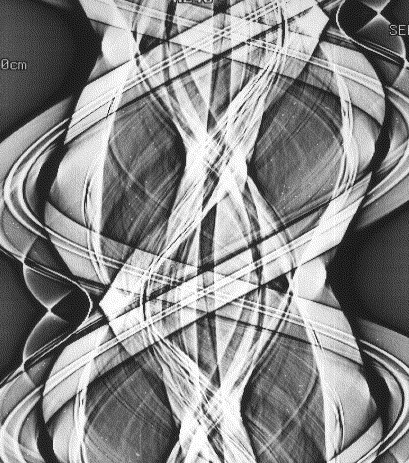
\includegraphics[scale=0.4]{sinogrammeExemple}
\caption[Exemple de sinogramme]{Exemple de sinogramme}
\label{fig:gallery}
\end{figure}

La transformée de Radon s'exprime par la relation suivante :
$R[f](u,\theta)=p_\theta(u)$
\\%
$=\int_{D_\theta} f(u\cos\theta-v\sin\theta, u\sin\theta+v\cos\theta)dv$

\textbf{A COMPLETER}

\subsection{La rétroprojection filtrée}

\textbf{A COMPLETER}


\section{Le code en pratique}

\subsection{le code Matlab}

\subsubsection{la génération de données }

L'objet d'étude que nous avons utilisés dans un premier temps sont les images d'un modèle humain, les fantômes de L. Shepp et B.F. Logan créée par  en 1974, qui sert de test pour les algorithmes de reconstructions.

Nous avons utilisés dans un premier temps comme objets d'étude les images d'un modèle humain appelés les fantômes de Shepp-Logan. Créée par ces derniers en 1974, qui servent de test pour les algorithmes de reconstructions (Fig.2).

\begin{figure}[H]
\centering
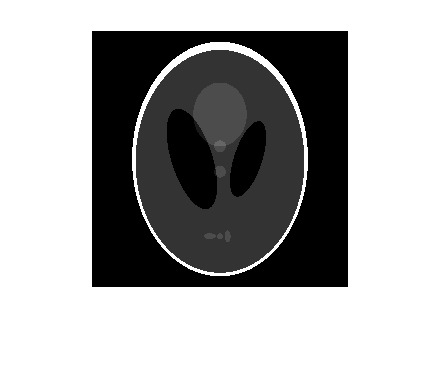
\includegraphics[scale=0.7]{Shepp-logan}
\caption[Fantômes de Shepp-Logan tels que générés par Matlab]{Fantômes de Shepp-Logan tels que générés par Matlab}
\label{fig:gallery}
\end{figure}

Pour modéliser la phase rayonnement pour obtenir le sinogramme sur lequel nous allons travailler pour la rétroprojection filtrée, nous avons appliqué la fonction Matlab de transformée de Radon. Cette fonction permet de choisir l'angle du rayonnement simulé ainsi que le nombre de mesures en faisant varier le pas de discrétisation.
En sortie de la transformée de Radon, nous obtenons une matrice R qui regroupe l'ensemble des mesures récoltées par angle de rayonnement simulé et un vecteur xp qui regroupe l'angle choisi pour chaque colonne. Le sinogramme ainsi obtenu est le suivant (Fig.3) :

\begin{figure}[H]
\centering
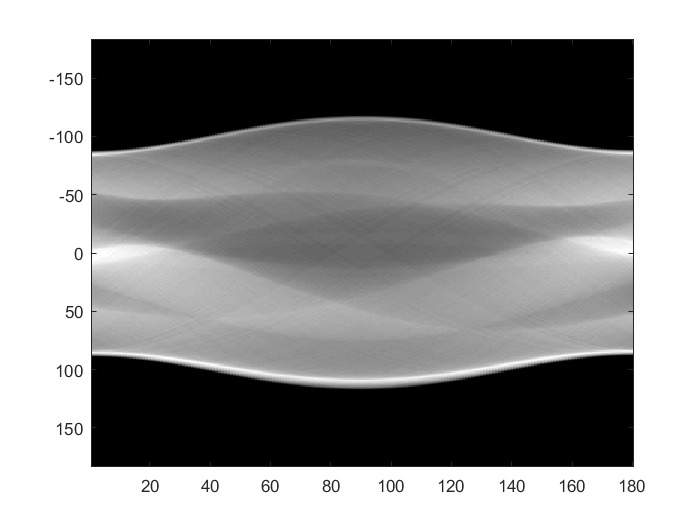
\includegraphics[scale=0.5]{sinogramme}
\caption[Sinogramme des fantômes de Shepp-Logan]{Sinogramme des fantômes de Shepp-Logan}
\label{fig:gallery}
\end{figure}



\subsubsection{rétroprojection discrète }

\textbf{Filtre de l'image :} La première étape est d'appliquer une transformée de Fourier à la matrice R résultante de la transformée de Radon de Matlab. Ensuite nous avons ensuite créé le filtre de Ram-Lak (Fig.4). \textbf{Explication pourquoi utiliser ce filtre et comment il marche.}

\begin{figure}[H]
\centering
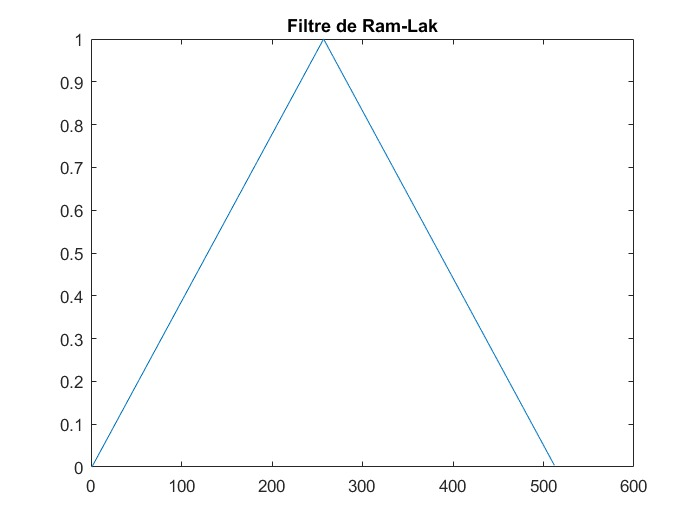
\includegraphics[scale=0.4]{filtre-de-Ram-Lak}
\caption[filtre de Ram-Lak]{filtre de Ram-Lak}
\label{fig:gallery}
\end{figure}

On applique le filtre à la matrice R par multiplication et appliquons au résultat une transformée de Fourier inverse.

\textbf{rétroprojection :} On crée une matrice B de la taille de R qui recueillera l'image résultat. En bouclant sur les colonnes de R, donc chaque angle de mesure, on détermine les projections $u$ avec la formule suivante :
$u=(((x-R_x)/2)*\cos(rad)-((y-R_y)/2)*\sin(rad))+xp_offset$
avec $(x,y)$ les points de B, $R_x$ et $R_y$ la taille de R, $rad$ l'angle en radian de l'axe de projection et $xp_offset$ le décalage.
Pour être sûr que les projections $u$ soient entières, nous appliquons une interpolation de Taylor.
Nous utilisons finalement une LUT pour restreindre les valeurs résultats dans l'ensemble [0;255].
On rappelle qu'une Look-Up Table (LUT) est utilisé en traitement d'image pour établir une correspondance entre les valeurs des points et les couleurs affichées.

\begin{figure}[H]
\centering
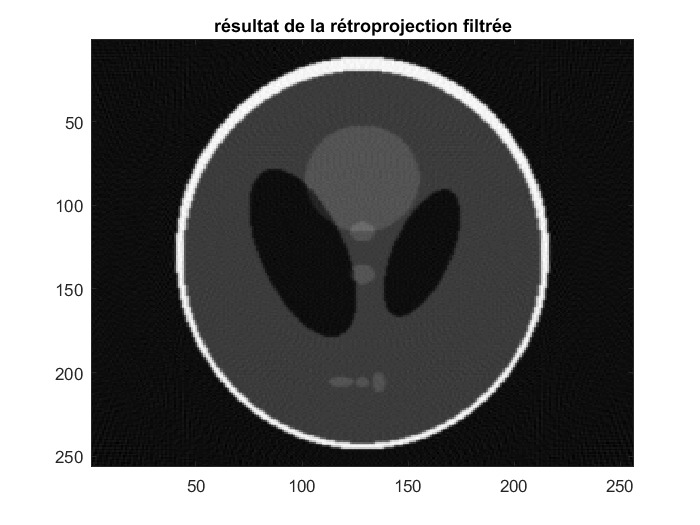
\includegraphics[scale=0.5]{rsultat-de-la-rtroprojetion-filtre}
	\caption[Résultat de la rétroprojection filtrée obtenus suite à notre code Matlab]{Résultat de la rétroprojection filtrée obtenus suite à notre code Matlab}
\label{fig:gallery}
\end{figure}



\subsubsection{quantification et évaluation des résultats}

Pour évaluer les images obtenus, nous avons utilisés le ratio PSNR (Peak Signal to Noise Ratio), qui se calcule de la manière suivante :
$PSNR=10\cdot\log_{10} (\frac{d^2}{EQM})$
où $EQM$ est l'erreur quadratique moyenne qui s'obtient par la formule suivante :
$EQM=\frac{1}{mn}\sum_{i=0}^{m-1}\sum_{j=0}^{n-1}(I_0(i,j)-I_f(i,j))^2$
où $I_0$ est l'image originale et $I_f$ l'image finale.
Ce ratio est la manière classique d'évaluer en traitement de l'image les distorsions par rapport à l'image d'origine.

Ainsi nous pouvons faire varier la qualité de l'image résultante de la rétroprojection en modifiant la taille de l'image en pixels ou le pas angulaire des rayonnements simulés.

\begin{figure}[H]
\centering
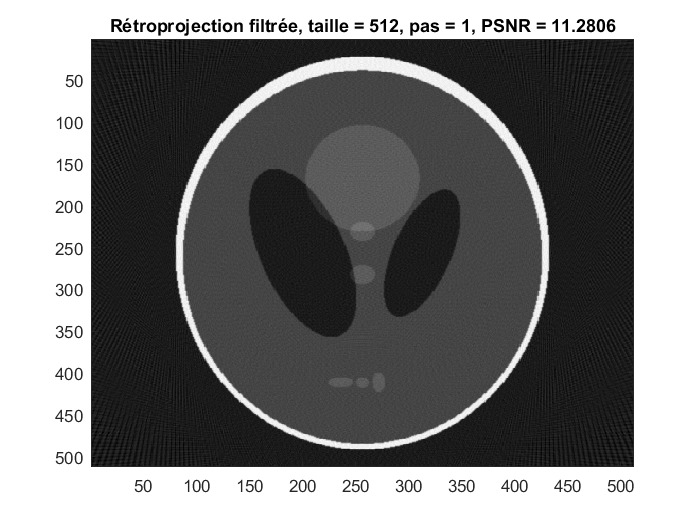
\includegraphics[scale=0.5]{t512-p1}
	\caption[Résultat taille=512 pas=1]{Résultat taille=512 pas=1}
\label{fig:gallery}
\end{figure}

Pour la Fig.6, on observe une image assez proche de l'original, avec un $PSNR=11.26$. Cette image est tout à fait interpretable par un humain, à la différence du sinogramme.

\begin{figure}[H]
\centering
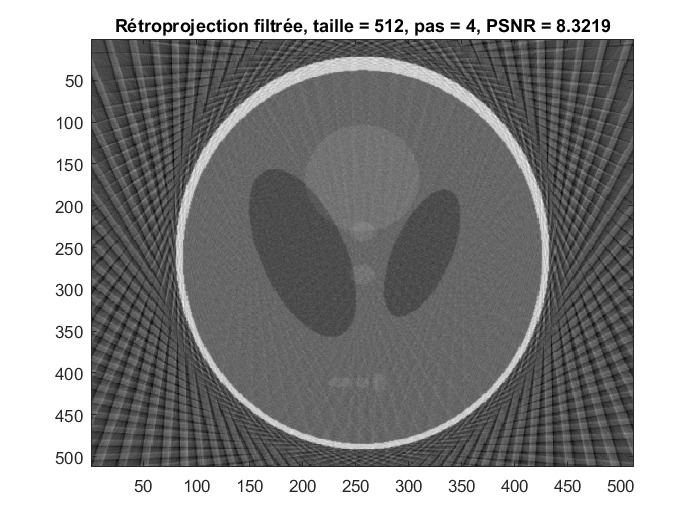
\includegraphics[scale=0.5]{t512-p4}
	\caption[Résultat taille=512 pas=4]{Résultat taille=512 pas=4}
\label{fig:gallery}
\end{figure}

Ici l'image de la Fig7. a un pas angulaire de 4. Des lignes parasites dù à un trop grand pas angulaire apparaissent. Le PSNR diminue à 8.32.

\begin{figure}[H]
\centering
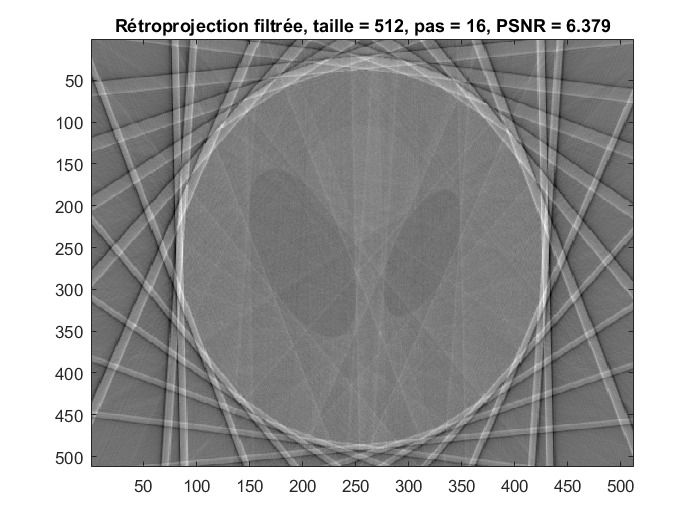
\includegraphics[scale=0.5]{t512-p16}
	\caption[Résultat taille=512 pas=16]{Résultat taille=512 pas=16}
\label{fig:gallery}
\end{figure}

En augmentant encore le pas angulaire jusqu'à 16, on observe que l'image de la Fig.8 devient quasiment inexploitable, qu'elle part nettement en contraste et que les lignes parasites sont encore plus nombreuses. Le PSNR chute à 6.37.


\begin{figure}[H]
\centering
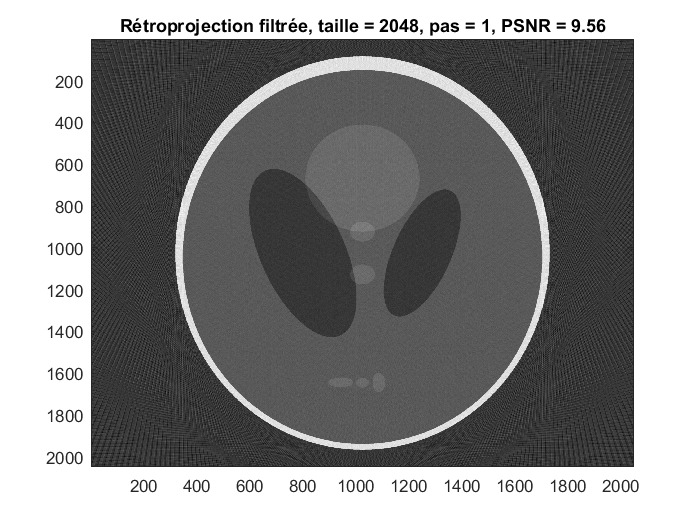
\includegraphics[scale=0.5]{t2048-p1}
	\caption[Résultat taille=2048 pas=1]{Résultat taille=2048 pas=1}
\label{fig:gallery}
\end{figure}

Finalement, cette image (Fig.9) a un pas angulaire de 1 comme la Fig.6, mais à une taille plus grande de 2048 pixels. Le PSNR de 9.56 est plus bas que la Fig.6, mais cela s'explique par le fait qu'on a augmenté la taille de l'image, sans pour autant augmenter le pas angulaire, aboutissant pour un même pas angulaire à un résultat moins efficace.

Le pas angulaire semble donc être le paramètre le plus sensible sur la qualité du rendu. Dés qu'on prends un pas angulaire supérieur à 1 radian, la dégradation de l'image s'accentue à toute vitesse.

\textbf{A COMPLETER, RAJOUTER GRAPHE PSNR et blabla à améliorer}


\subsection{le code C}

Le code C que nous avons écrits et équivalent algorithmiquement au code Matlab. Notre plus grande difficultés fut de remplacer des fonctions pré établi dans Matlab par des libraires équivalentes.

\textbf{A COMPLETER}


% An example of a floating figure using the graphicx package.
% Note that \label must occur AFTER (or within) \caption.
% For figures, \caption should occur after the \includegraphics.
% Note that IEEEtran v1.7 and later has special internal code that
% is designed to preserve the operation of \label within \caption
% even when the captionsoff option is in effect. However, because
% of issues like this, it may be the safest practice to put all your
% \label just after \caption rather than within \caption{}.
%
% Reminder: the "draftcls" or "draftclsnofoot", not "draft", class
% option should be used if it is desired that the figures are to be
% displayed while in draft mode.
%
%\begin{figure}[!t]
%\centering
%\includegraphics[width=2.5in]{myfigure}
% where an .eps filename suffix will be assumed under latex, 
% and a .pdf suffix will be assumed for pdflatex; or what has been declared
% via \DeclareGraphicsExtensions.
%\caption{Simulation results for the network.}
%\label{fig_sim}
%\end{figure}

% Note that the IEEE typically puts floats only at the top, even when this
% results in a large percentage of a column being occupied by floats.


% An example of a double column floating figure using two subfigures.
% (The subfig.sty package must be loaded for this to work.)
% The subfigure \label commands are set within each subfloat command,
% and the \label for the overall figure must come after \caption.
% \hfil is used as a separator to get equal spacing.
% Watch out that the combined width of all the subfigures on a 
% line do not exceed the text width or a line break will occur.
%
%\begin{figure*}[!t]
%\centering
%\subfloat[Case I]{\includegraphics[width=2.5in]{box}%
%\label{fig_first_case}}
%\hfil
%\subfloat[Case II]{\includegraphics[width=2.5in]{box}%
%\label{fig_second_case}}
%\caption{Simulation results for the network.}
%\label{fig_sim}
%\end{figure*}
%
% Note that often IEEE papers with subfigures do not employ subfigure
% captions (using the optional argument to \subfloat[]), but instead will
% reference/describe all of them (a), (b), etc., within the main caption.
% Be aware that for subfig.sty to generate the (a), (b), etc., subfigure
% labels, the optional argument to \subfloat must be present. If a
% subcaption is not desired, just leave its contents blank,
% e.g., \subfloat[].


% An example of a floating table. Note that, for IEEE style tables, the
% \caption command should come BEFORE the table and, given that table
% captions serve much like titles, are usually capitalized except for words
% such as a, an, and, as, at, but, by, for, in, nor, of, on, or, the, to
% and up, which are usually not capitalized unless they are the first or
% last word of the caption. Table text will default to \footnotesize as
% the IEEE normally uses this smaller font for tables.
% The \label must come after \caption as always.
%
%\begin{table}[!t]
%% increase table row spacing, adjust to taste
%\renewcommand{\arraystretch}{1.3}
% if using array.sty, it might be a good idea to tweak the value of
% \extrarowheight as needed to properly center the text within the cells
%\caption{An Example of a Table}
%\label{table_example}
%\centering
%% Some packages, such as MDW tools, offer better commands for making tables
%% than the plain LaTeX2e tabular which is used here.
%\begin{tabular}{|c||c|}
%\hline
%One & Two\\
%\hline
%Three & Four\\
%\hline
%\end{tabular}
%\end{table}


% Note that the IEEE does not put floats in the very first column
% - or typically anywhere on the first page for that matter. Also,
% in-text middle ("here") positioning is typically not used, but it
% is allowed and encouraged for Computer Society conferences (but
% not Computer Society journals). Most IEEE journals/conferences use
% top floats exclusively. 
% Note that, LaTeX2e, unlike IEEE journals/conferences, places
% footnotes above bottom floats. This can be corrected via the
% \fnbelowfloat command of the stfloats package.




\section{Conclusion}

Comme expliqué dans cet article, nous avons appliqué une « rétroprojection filtrée » d’abord sur des exemples théoriques (disque) et l’avons ensuite implémentée en Matlab, puis en langage C. Enfin, notre code fut appliqué sur les fantômes de Shepp-Logann en fesant varier le pas angulaire et la dimension de l'image. Les PNSR varie pour un pas de 1 radian entre 12.41 pour une image de 64 pixels et 9.56 une image de 2048 pixels et varie pour une image à 512 pixels entre 11.28 pour un pas de 1 et 6.1 pour un pas de radian. On remarque aussi que le pas augulaire joue beaucoup plus sur l'interprétation humaine de l'image résultante que la dimension de l'image. Les temps de calculs sont prohibitifs dès que les dimensions des images calculés deviennent très importantes. En effet, pour un test sur des images de .... pixels, nous avons pris près de 8h pour effectuer l'ensemble des calculs (rétroprojection+PSNR). Notre code doit être optimisé si l'on veut l'appliquer à des images conséquentes et reste à tester sur des sinogrammes d'acquisition d'objets d'études réels. 
\\
L'étude de la tomographie et de la rétroprojection filtrée fut instructives pour nous lors de la réalisation de ce PIDR.

\textbf{A compléter}




% conference papers do not normally have an appendix


% use section* for acknowledgment
\section*{Remerciement}

Nous tenons à remercier notre encadrant PIDR, qui a été présent durant ces 5 mois d'étude pour répondre à nos questions, nous conseiller sur certains choix à prendre. Son expertise dans le domaine de la tomographie a su nous orienter lors de la quinzaine de réunion téléphonique que nous avons eu les mercredis de cette année. Le sujet qu'il nous a proposé fut riche d'enseignement et instructif pour nous deux.


% trigger a \newpage just before the given reference
% number - used to balance the columns on the last page
% adjust value as needed - may need to be readjusted if
% the document is modified later
%\IEEEtriggeratref{8}
% The "triggered" command can be changed if desired:
%\IEEEtriggercmd{\enlargethispage{-5in}}

% references section
\newpage
% can use a bibliography generated by BibTeX as a .bbl file
% BibTeX documentation can be easily obtained at:
% http://mirror.ctan.org/biblio/bibtex/contrib/doc/
% The IEEEtran BibTeX style support page is at:
% http://www.michaelshell.org/tex/ieeetran/bibtex/
%\bibliographystyle{IEEEtran}
% argument is your BibTeX string definitions and bibliography database(s)
%\bibliography{IEEEabrv,../bib/paper}
%
% <OR> manually copy in the resultant .bbl file
% set second argument of \begin to the number of references
% (used to reserve space for the reference number labels box)
\begin{thebibliography}{1}

\bibitem{IEEEhowto:kopka}
Papa et Maman, \emph{Notre Fils est génial !! \LaTeX}, 3rd~ed.\hskip 1em plus
  0.5em minus 0.4em\relax Paris, France: ..., 2017

\end{thebibliography}




% that's all folks
\end{document}


